\documentclass[journal]{IEEEtran}

\usepackage{mathptmx}
\usepackage{amsmath}
\usepackage{booktabs}
\usepackage{multirow}
\usepackage{array}
\usepackage{graphicx}
\usepackage{placeins}
\usepackage{url}
\usepackage{listings}
\usepackage{xcolor}
\lstset{linewidth=0.95\columnwidth}

\lstdefinelanguage{json}{
    basicstyle=\ttfamily\small,
    numbers=left,
    numberstyle=\tiny,
    stepnumber=1,
    numbersep=5pt,
    showstringspaces=false,
    breaklines=true,
    frame=single,
    backgroundcolor=\color{white},
    literate=
     *{0}{{{\color{blue}0}}}{1}
      {1}{{{\color{blue}1}}}{1}
      {2}{{{\color{blue}2}}}{1}
      {3}{{{\color{blue}3}}}{1}
      {4}{{{\color{blue}4}}}{1}
      {5}{{{\color{blue}5}}}{1}
      {6}{{{\color{blue}6}}}{1}
      {7}{{{\color{blue}7}}}{1}
      {8}{{{\color{blue}8}}}{1}
      {9}{{{\color{blue}9}}}{1}
      {:}{{{\color{red}:}}}{1}
      {,}{{{\color{red},}}}{1}
      {\{}{{{\color{black}{\{}}}}{1}
      {\}}{{{\color{black}{\}}}}}{1}
      {[}{{{\color{black}{[}}}}{1}
      {]}{{{\color{black}{]}}}}{1},
}

% Suppress warnings when multiple PDFs with page groups are included on the same page
\pdfsuppresswarningpagegroup=1
% Ensure compatibility with transparency groups in included PDFs (optional but helps)
\pdfminorversion=7

% Fix for DOI font - use normal font for URLs to avoid slashed zero
\urlstyle{rm}

% SVG FILES HAVE BEEN CONVERTED TO PDF FORMAT
% All 60 visualization examples (40 training + 20 test) are now included in the document
% PDF files are located in Train_set/ and Test_set/ directories

\title{Supplemental Material: Chart Selection Criteria and Dataset Description}

\begin{document}

\twocolumn[
{\centering
{\Large\textbf{SUPPLEMENTAL MATERIAL}}\\[0.5em]
{\Large\textbf{Chart Selection Criteria and Dataset Description}}\\[1em]
}
]

Our dataset contains 60 SVG visualization examples, 40 of which are used exclusively for training and 20 for testing. This supplementary material documents our dataset construction methodology, graph selection criteria, theoretical complexity analysis framework, test dataset statistics to support evaluation methods, and a questionnaire annotation system for manually annotating these datasets.

\section{Dataset Collection}

\subsection{Source Selection and Coverage}

We collected charts from three authoritative platforms: D3.js official examples (industry-standard interactive visualizations), Highcharts gallery (professional charting samples), and Plotly examples (cross-platform references). This multi-platform approach ensures diversity across real-world visualization practices and follows established perceptual guidelines~\cite{cleveland1984}.

Our chart selection follows established visualization taxonomy based on \textit{A Guide to Choosing the Right Chart Type}~\cite{szoka1982}. Table~\ref{tab:chart_taxonomy} presents the comprehensive categorization framework that guided our dataset construction, ensuring systematic coverage across fundamental data relationship types.

\begin{table}[!htb]
\centering
\caption{Chart Taxonomy and Coverage Framework}
\label{tab:chart_taxonomy}
\footnotesize
\begin{tabular}{p{2.5cm}p{5.2cm}}
\toprule
\textbf{Data Type} & \textbf{Corresponding Chart Types} \\
\midrule
\textbf{Time Series} & Curve chart, Double-scale curve, Column chart, Surface chart, Step chart \\
\midrule
\textbf{Parts of Whole} & Pie chart, 100\% column chart, 100\% bar chart \\
\midrule
\textbf{Multiple Objects} & Bar chart, Column chart, Sorted bar, Floating bar, Patch map, Pictogram \\
\midrule
\textbf{Variable Relations} & Scatter plot, Scatter-and-line plot, Dual bar, Pyramid chart, Curve chart \\
\bottomrule
\end{tabular}
\end{table}

% \subsection{Complexity-based Selection}
% (Content moved to Section "Dataset Construction")
% Chart complexity is defined through visual element count (graphical primitives), visual channel count (encoding dimensions), and integrated complexity score (weighted combination based on cognitive load theory~\cite{cowan2001}). For the training set, we used uniform sampling, taking approximately 25\% of the samples in each of the low, medium, high, and very high complexity levels to ensure balanced representation. However, for the test set, we deliberately employed non-uniform sampling with intentional bias toward higher complexity levels (40\% highly complex vs 22.5\% in training) to create a more challenging evaluation scenario that better assesses model performance under demanding conditions and provides stronger discriminative power for algorithm comparison.
% 
% Quality assurance involved filtering charts with overlapping elements, inconsistent data-visual mappings, excessive cognitive load, and perceptual validity issues. Color encoding strategies include monochromatic, analogous, complementary, sequential, and diverging schemes to enhance generalization~\cite{bertin1967}.

\subsection{Rationale for Removing legend and axis labels}
Prior to feature extraction and complexity analysis, we manually removed numerical axes, coordinate grids, and legends from every collected SVG file. This preprocessing step is motivated by two complementary considerations:

\begin{enumerate}
    \item \textbf{Visualization simplification.} Although axes and legends are indispensable for human interpretation, their concrete visual forms (tick styles, label density, legend placement, etc.) vary substantially across charting libraries. These variations contribute little to the geometric or topological structure that determines the saliency of data patterns. Removing them therefore reduces annotation effort, alleviates model learning burden, and allows the remaining visual bandwidth to be devoted to core graphical primitives (bars, lines, areas, nodes, links, \emph{etc.}).
    \item \textbf{Enhanced pattern perception.} In interactive studies of pattern saliency, auxiliary annotation elements can distract attention away from the key visual patterns of interest. Eliminating axes and legends encourages both human observers and automated models to focus on the intrinsic shapes and spatial arrangements that convey the underlying data relationships, thereby improving the sensitivity of subsequent complexity evaluation.
\end{enumerate}

This simplification strategy follows the principle of isolating essential visual signals while discarding redundant decorations, ultimately leading to a cleaner dataset and more robust assessment of pattern salience.

\subsection{Complexity-based Selection}
After collecting a large amount of SVG data and preprocessing them to remove the axes and legends, we selected them by Chart complexity. Chart complexity is defined through visual element count (graphical primitives), visual channel count (encoding dimensions), and integrated complexity score (weighted combination based on cognitive load theory~\cite{cowan2001}). For the training set, we used uniform sampling, taking approximately 25\% of the samples in each of the low, medium, high, and very high complexity levels to ensure balanced representation. However, for the test set, we deliberately employed non-uniform sampling with intentional bias toward higher complexity levels (40\% highly complex vs 22.5\% in training) to create a more challenging evaluation scenario that better assesses model performance under demanding conditions and provides stronger discriminative power for algorithm comparison.

Additionally, we performed quality assurance to filter out charts with overlapping elements, inconsistent data-visual mappings, excessive cognitive load, and perceptual validity issues. Color encoding strategies include monochromatic, analogous, complementary, sequential, and diverging schemes to enhance generalization~\cite{bertin1967}.

\subsection{Theoretical Complexity Framework}
Our framework integrates established theories from cognitive science and perceptual psychology~\cite{cleveland1984,cowan2001,stevens1957}.

\textbf{Cleveland-McGill Perceptual Hierarchy~\cite{cleveland1984}:} Different visual encodings receive accuracy-based weights:
\begin{align}
w_{\text{position}} &= 1.0, \quad w_{\text{length}} = 1.2, \quad w_{\text{angle}} = 1.8 \nonumber \\
w_{\text{area}} &= 2.4, \quad w_{\text{color}} = 3.2
\end{align}

\textbf{Cognitive Load Theory~\cite{cowan2001}:} Based on working memory limitations:
\begin{equation}
C_{\text{cognitive}} = \begin{cases}
0 & \text{if } n \leq 4 \\
\left(\frac{n-4}{4}\right)^{1.5} \times 3.0 & \text{if } n > 4
\end{cases}
\end{equation}

\textbf{Stevens' Power Law~\cite{stevens1957}:} For color perception complexity:
\begin{equation}
C_{\text{color}} = n_{\text{color}}^{0.4} \times 2.5 \times 1.5
\end{equation}

\textbf{Integrated Score:} Final complexity combines all dimensions:
\begin{align}
C_{\text{total}} &= C_{\text{element}} \times 1.0 + C_{\text{channel}} \times 2.0 \nonumber \\
&\quad + C_{\text{color}} \times 1.5 + C_{\text{cognitive}} \times 3.0 \nonumber \\
&\quad + C_{\text{transform}} \times 1.2
\end{align}


\section{Dataset Description}

\subsection{Training and Test Set Comparison}

Figures~\ref{fig:training_complexity} and \ref{fig:test_complexity} provide detailed visualization of complexity distributions across both datasets, showing significant complexity differences between training and test sets. The test set exhibits higher mean complexity (934.5 vs 463.3, p<0.001) and greater emphasis on challenging visualizations, validating our evaluation design.

\begin{figure}[!htb]
\centering
\includegraphics[width=\columnwidth]{training_set_complexity_analysis.pdf}
\caption{Training Set Complexity Analysis: Distribution of complexity scores across chart types showing balanced representation across difficulty levels.}
\label{fig:training_complexity}
\end{figure}

\begin{figure}[!htb]
\centering
\includegraphics[width=\columnwidth]{test_set_complexity_analysis.pdf}
\caption{Test Set Complexity Analysis: Distribution emphasizing higher complexity scenarios with 40\% highly complex visualizations for rigorous evaluation.}
\label{fig:test_complexity}
\end{figure}

\subsubsection{File-by-File Description}
Tables~\ref{tab:training_details} and \ref{tab:test_details} provide comprehensive complexity analysis for all 60 dataset files. The training set demonstrates complexity scores ranging from 50.8 to 4,684.0 points across diverse chart types, ensuring balanced coverage across difficulty levels. The test set strategically emphasizes challenging visualization scenarios with complexity scores reaching up to 6,627.5 points, providing robust evaluation benchmarks.

\begin{table}[!htbp]
  \centering
  \caption{Test Set Complete Analysis}
  \label{tab:test_details}
  \scriptsize
  \begin{tabular}{p{0.6cm}p{1.9cm}r@{\hspace{0.25cm}}r@{\hspace{0.25cm}}r@{\hspace{0.3cm}}p{1.7cm}}
  \toprule
  \textbf{File} & \textbf{Category} & \textbf{Elem.} & \textbf{Ch.} & \textbf{Score} & \textbf{Chart Type} \\
  \midrule
  1.svg & Complex & 70 & 7 & 391.6 & Complex \\
  2.svg & Medium & 36 & 4 & 136.6 & Standard \\
  3.svg & Highly Complex & 201 & 3 & 1752.6 & High Complex \\
  4.svg & Complex & 64 & 4 & 332.2 & Path Chart \\
  5.svg & Medium & 22 & 3 & 102.3 & Standard \\
  6.svg & Medium & 29 & 3 & 136.5 & Standard \\
  7.svg & Highly Complex & 332 & 3 & 3304.1 & Path Chart \\
  8.svg & Highly Complex & 169 & 3 & 1195.8 & Path Chart \\
  9.svg & Simple & 14 & 5 & 84.1 & Basic Chart \\
  10.svg & Highly Complex & 589 & 3 & 6627.5 & Path Chart \\
  11.svg & Medium & 21 & 3 & 103.5 & Standard \\
  12.svg & Medium & 25 & 4 & 127.9 & Standard \\
  13.svg & Medium & 30 & 4 & 146.9 & Standard \\
  14.svg & Medium & 34 & 5 & 175.5 & Network \\
  15.svg & Highly Complex & 171 & 3 & 1214.1 & Path Chart \\
  16.svg & Highly Complex & 130 & 6 & 767.5 & Network \\
  17.svg & Highly Complex & 145 & 5 & 953.0 & Network \\
  18.svg & Complex & 74 & 5 & 374.6 & Complex \\
  19.svg & Complex & 43 & 3 & 213.1 & Path Chart \\
  20.svg & Highly Complex & 97 & 4 & 550.1 & Complex \\
  \bottomrule
  \multicolumn{6}{l}{\textbf{Summary:} Mean Elements: 114.8, Mean Score: 934.5} \\
  \end{tabular}
  \end{table}

\begin{table}[!t]
\centering
\caption{Training Set Complete Analysis}
\label{tab:training_details}
\scriptsize
\begin{tabular}{p{0.6cm}p{1.9cm}r@{\hspace{0.25cm}}r@{\hspace{0.25cm}}r@{\hspace{0.3cm}}p{1.7cm}}\toprule
\textbf{File} & \textbf{Category} & \textbf{Elem.} & \textbf{Ch.} & \textbf{Score} & \textbf{Chart Type} \\
\midrule

1.svg & Complex & 81 & 4 & 366.3 & Scatter Plot \\
2.svg & Complex & 77 & 4 & 347.4 & Dense Bar \\
3.svg & Highly Complex & 252 & 4 & 1772.5 & Dense Bar \\
4.svg & Simple & 17 & 4 & 64.2 & Basic Chart \\
5.svg & Medium & 52 & 2 & 201.5 & Standard \\
6.svg & Medium & 32 & 3 & 143.0 & Standard \\
7.svg & Simple & 12 & 4 & 50.8 & Basic Chart \\
8.svg & Simple & 19 & 3 & 93.0 & Color-Rich \\
9.svg & Medium & 34 & 3 & 163.2 & Path Chart \\
10.svg & Simple & 15 & 4 & 81.0 & Basic Chart \\
11.svg & Complex & 70 & 3 & 386.5 & Path Chart \\
12.svg & Highly Complex & 497 & 4 & 4684.0 & Dense Bar \\
13.svg & Complex & 46 & 5 & 212.1 & Multi-Variate \\
14.svg & Simple & 15 & 4 & 62.4 & Basic Chart \\
15.svg & Highly Complex & 80 & 5 & 533.3 & Complex \\
16.svg & Medium & 46 & 2 & 187.3 & Standard \\
17.svg & Simple & 18 & 4 & 91.1 & Basic Chart \\
18.svg & Complex & 73 & 4 & 394.0 & Path Chart \\
19.svg & Highly Complex & 258 & 4 & 2093.8 & Path Chart \\
20.svg & Highly Complex & 81 & 4 & 468.7 & Path Chart \\
21.svg & Medium & 25 & 4 & 94.9 & Standard \\
22.svg & Simple & 15 & 4 & 62.9 & Basic Chart \\
23.svg & Complex & 53 & 4 & 216.7 & Complex \\
24.svg & Simple & 15 & 5 & 92.7 & Basic Chart \\
25.svg & Medium & 19 & 4 & 98.9 & Color-Rich \\
26.svg & Highly Complex & 145 & 4 & 822.6 & Tree Map \\
27.svg & Complex & 70 & 4 & 384.8 & Path Chart \\
28.svg & Highly Complex & 160 & 3 & 988.8 & Tree Map \\
29.svg & Simple & 16 & 5 & 73.3 & Basic Chart \\
30.svg & Medium & 44 & 5 & 206.4 & Multi-Variate \\
31.svg & Simple & 14 & 4 & 77.0 & Basic Chart \\
32.svg & Complex & 61 & 5 & 282.2 & Complex \\
33.svg & Highly Complex & 155 & 3 & 1054.3 & Bubble \\
34.svg & Complex & 54 & 5 & 294.1 & Network \\
35.svg & Highly Complex & 114 & 3 & 587.8 & Dense Bar \\
36.svg & Medium & 24 & 5 & 129.2 & Multi-Variate \\
37.svg & Complex & 75 & 4 & 366.0 & Complex \\
38.svg & Medium & 23 & 4 & 110.9 & Standard \\
39.svg & Medium & 33 & 5 & 129.5 & Bubble \\
40.svg & Simple & 12 & 3 & 63.6 & Color-Rich \\
\bottomrule
\multicolumn{6}{l}{\textbf{Summary:} Mean Elements: 72.5, Mean Score: 463.3} \\
\end{tabular}
\end{table}

\subsubsection{Dataset Overview}

The complete dataset comprises 60 carefully curated visualization examples distributed across training and test sets with deliberate complexity stratification. Detailed visual documentation of all dataset components is provided in the visual examples section below for comprehensive reference.

\subsubsection{Questionnaire Annotation System}

Figure~\ref{fig:questionnaire_ui_a} to \ref{fig:questionnaire_ui_d} illustrates the four key screens of our web-based questionnaire annotation platform. The workflow is as follows:
\begin{enumerate}
    \item \textbf{Landing page (Fig.~\ref{fig:questionnaire_ui_a}).} Annotators first enter their personal information (completely confidential) and select their level of proficiency in creating visualizations. This step generates a unique session token used to track progress for each annotator.
    \item \textbf{Interactive novice guide (Fig.~\ref{fig:questionnaire_ui_b}).} Annotators then learn how to use the annotation system through an interactive step-by-step onboarding tutorial.
    \item \textbf{Annotation interface (Figure~\ref{fig:questionnaire_ui_c}). } After completing the novice guide, the annotator officially enters the annotation interface. The left upper panel dynamically renders the target SVG visualization effect, while the annotator selects elements through the lower left panel (supports box selection and sliding selection), and the right panel displays the elements used for group creation, existing elements in the group, and perceived complexity scores. The progress bar at the bottom indicates the remaining tasks (the data that each annotator needs to annotate is 10 SVG examples randomly selected from the dataset).
    \item \textbf{Submission confirmation (Figure~\ref{fig:questionnaire_ui_d}). } After each submission, the system will upload the data to the server for processing. Annotators will receive immediate feedback and receive compensation based on their unique session token.
\end{enumerate}
All collected annotations are aggregated into a CSV file and processed into a special format for downstream analysis and model training.
% ------------------- questionnaire UI figure -------------------
\begin{figure}[!htbp]
    \centering
    \includegraphics[width=0.95\columnwidth]{questionnaire/1.pdf}
    \caption{Landing page of the questionnaire annotation system.}
    \label{fig:questionnaire_ui_a}
\end{figure}

\begin{figure}[!htbp]
    \centering
    
\includegraphics[width=0.95\columnwidth]{questionnaire/3.pdf}
    \caption{Interactive novice guide of the questionnaire annotation system.}
    \label{fig:questionnaire_ui_b}
\end{figure}

\begin{figure}[!htbp]
    \centering
    
\includegraphics[width=0.95\columnwidth]{questionnaire/10.pdf}
    \caption{Annotation interface of the questionnaire annotation system.}
    \label{fig:questionnaire_ui_c}
\end{figure}

\begin{figure}[!htbp]
  \centering
  
\includegraphics[width=0.95\columnwidth]{questionnaire/11.pdf}
  \caption{Submission confirmation screen of the questionnaire annotation system.}
  \label{fig:questionnaire_ui_d}
\end{figure}


\bibliographystyle{IEEEtran}
\begin{thebibliography}{9}

\bibitem{cleveland1984}
W.~S. Cleveland and R.~McGill.
\newblock Graphical perception: Theory, experimentation, and application to the development of graphical methods.
\newblock \emph{Journal of the American Statistical Association}, 79(387):531--554, 1984.
\newblock \url{https://doi.org/10.1080/01621459.1984.10478080}

\bibitem{szoka1982}
K.~Szoka.
\newblock A guide to choosing the right chart type.
\newblock \emph{IEEE Transactions on Professional Communication}, (2):98--101, 1982.
\newblock \url{https://doi.org/10.1109/TPC.1982.6447763}

\bibitem{bertin1967}
J.~Bertin.
\newblock \emph{Semiology of graphics: Diagrams, networks, maps}.
\newblock University of Wisconsin Press, 1967.
\newblock ISBN: 9780299061500

\bibitem{cowan2001}
N.~Cowan.
\newblock The magical number 4 in short-term memory: A reconsideration of mental storage capacity.
\newblock \emph{Behavioral and Brain Sciences}, 24(1):87--114, 2001.
\newblock \url{https://doi.org/10.1017/S0140525X01003922}

\bibitem{stevens1957}
S.~S. Stevens.
\newblock On the psychophysical law.
\newblock \emph{Psychological Review}, 64(3):153--181, 1957.
\newblock \url{https://doi.org/10.1037/h0046162}

\end{thebibliography}


\clearpage
\textbf{Initial Annotation Data Format}

The following is an example of the initial annotation data format in JSON, which describes the initial data structure for the questionnaire annotation system, including basic information, annotation steps, groups, and their ratings.

\begin{lstlisting}[language=json]
{
  "formData": {
    "studentid": "studentid",
    "age": "age",
    "gender": "gender",
    "visualimpairment": "yes/no",
    "visualizationExperience": "yes/no",
    "id": "unique session token"
  },
  "startTime": "startTime",
  "endTime": "endTime",
  "duration": "duration (endTime - startTime) in seconds",
  "steps": [
    {
      "stepId": stepId (corresponding absolute id in the dataset),
      "groups": [
        {
          "group": "group_1",
          "nodes": ["rect_10", "circle_7", "rect_1", "rect_4"],
          "ratings": {
            "attention": 3,
            "correlation_strength": 2,
            "exclusionary_force": 1
          }
        },
        {
          "group": "group_2",
          "nodes": ["path_2", "rect_5", "rect_8", "rect_11"],
          "ratings": {
            "attention": 2,
            "correlation_strength": 2,
            "exclusionary_force": 2
          }
        },
        {
          "group": "group_3",
          "nodes": ["path_9", "circle_6", "path_3", "path"],
          "ratings": {
            "attention": 3,
            "correlation_strength": 2,
            "exclusionary_force": 1
          }
        },
        {
          "group": "group_4",
          "nodes": ["rect_10", "path_7"],
          "ratings": {
            "attention": 3,
            "correlation_strength": 2,
            "exclusionary_force": 1
          }
        }
      ]
    }
    // ... (subsequent group data)
  ]
}
\end{lstlisting}


\textbf{Final Annotation Data Format}

The following is an example of the final annotation data format in JSON, which describes the final data structure for training and testing.

\begin{lstlisting}[language=json]
{
    "all_features": [
      [
        feature_1,
        feature_2,
        feature_3,
        feature_4,
        feature_5,
        feature_6,
        feature_7,
        ... (other features)
        feature_23,
      ],
      // ... (other features of other elements data)
    ],
    "groups": [
    [
      [
        feature_1,
        feature_2,
        feature_3,
        feature_4,
        feature_5,
        feature_6,
        feature_7,
        ... (other features)
        feature_23,
      ],
      // ... (other features of elements data in the group)
    ]
[

\end{lstlisting}


\clearpage

\textbf{Training Set}

The following figures present all 40 training set visualizations ordered by filename for comprehensive reference and transparency.


\vspace{1em}

\begin{figure}[!htbp]
\centering
\begin{minipage}{0.233\columnwidth}
\centering
\includegraphics[width=\textwidth]{Train_set/1.pdf}
{1.svg (366.3)}
\end{minipage}
\hfill
\begin{minipage}{0.233\columnwidth}
\centering
\includegraphics[width=\textwidth]{Train_set/2.pdf}
{2.svg (347.4)}
\end{minipage}
\hfill
\begin{minipage}{0.233\columnwidth}
\centering

\includegraphics[width=\textwidth]{Train_set/3.pdf}
{3.svg (1772.5)}
\end{minipage}
\hfill
\begin{minipage}{0.233\columnwidth}
\centering
\includegraphics[width=\textwidth]{Train_set/4.pdf}
{4.svg (64.2)}
\end{minipage}
\end{figure}

\begin{figure}[!htbp]
\centering
\begin{minipage}{0.233\columnwidth}
\centering
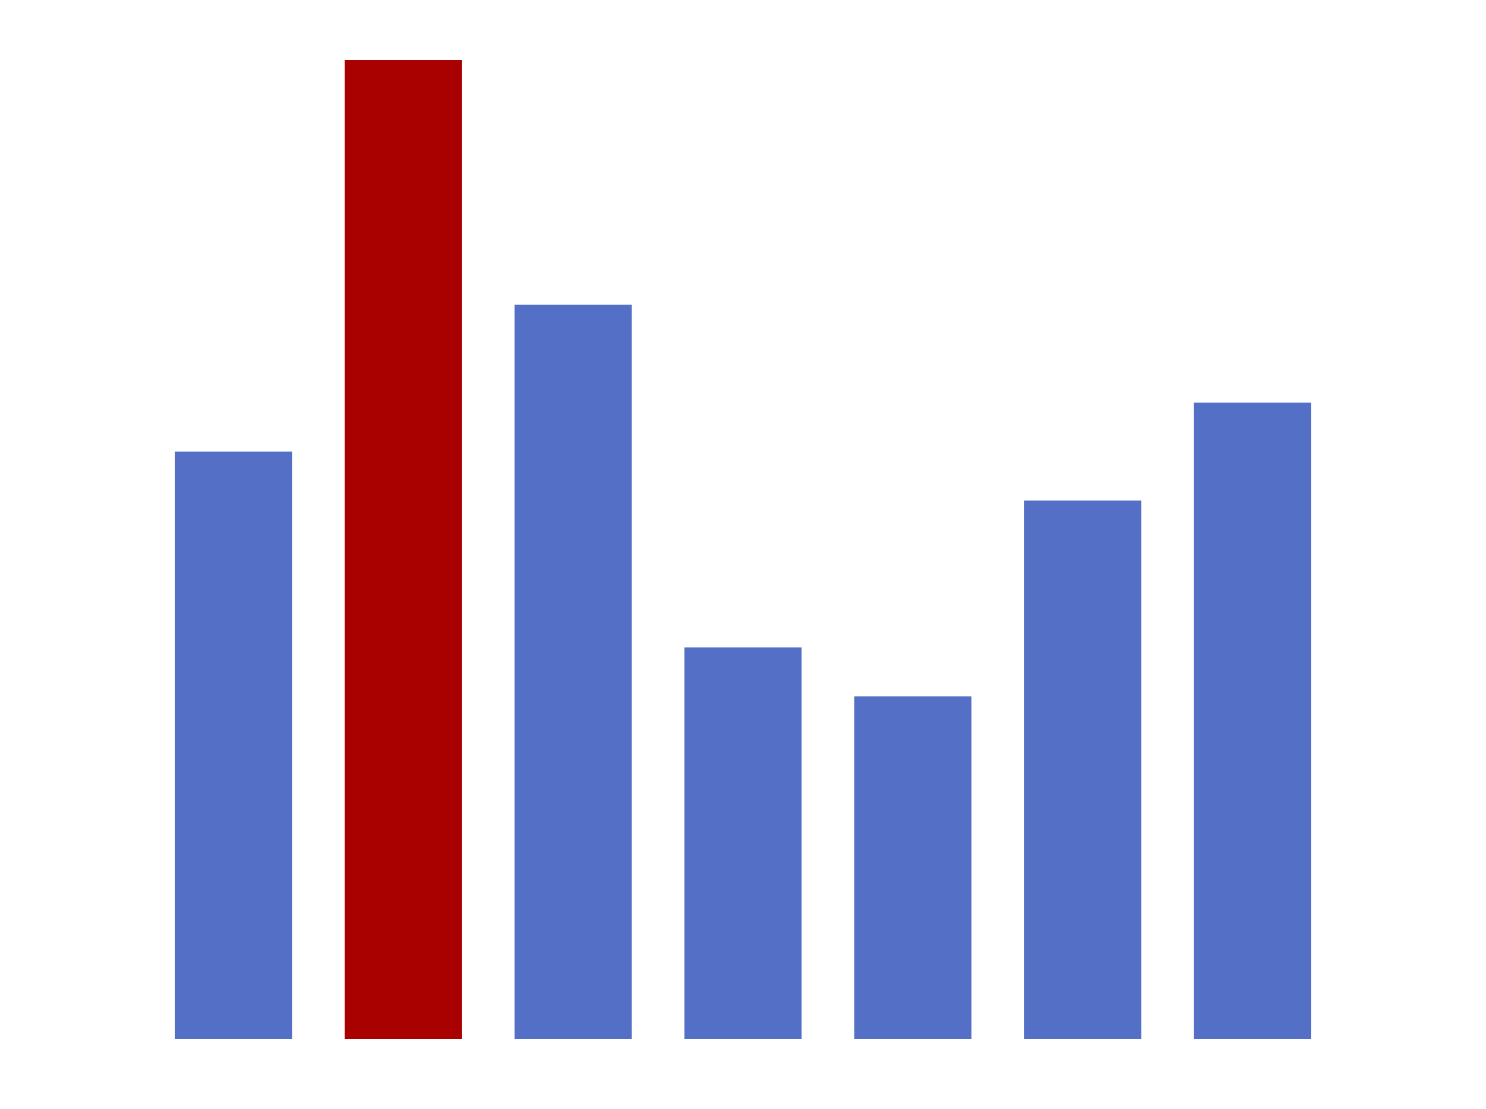
\includegraphics[width=\textwidth]{Train_set/5.pdf}
{5.svg (201.5)}
\end{minipage}
\hfill
\begin{minipage}{0.233\columnwidth}
\centering
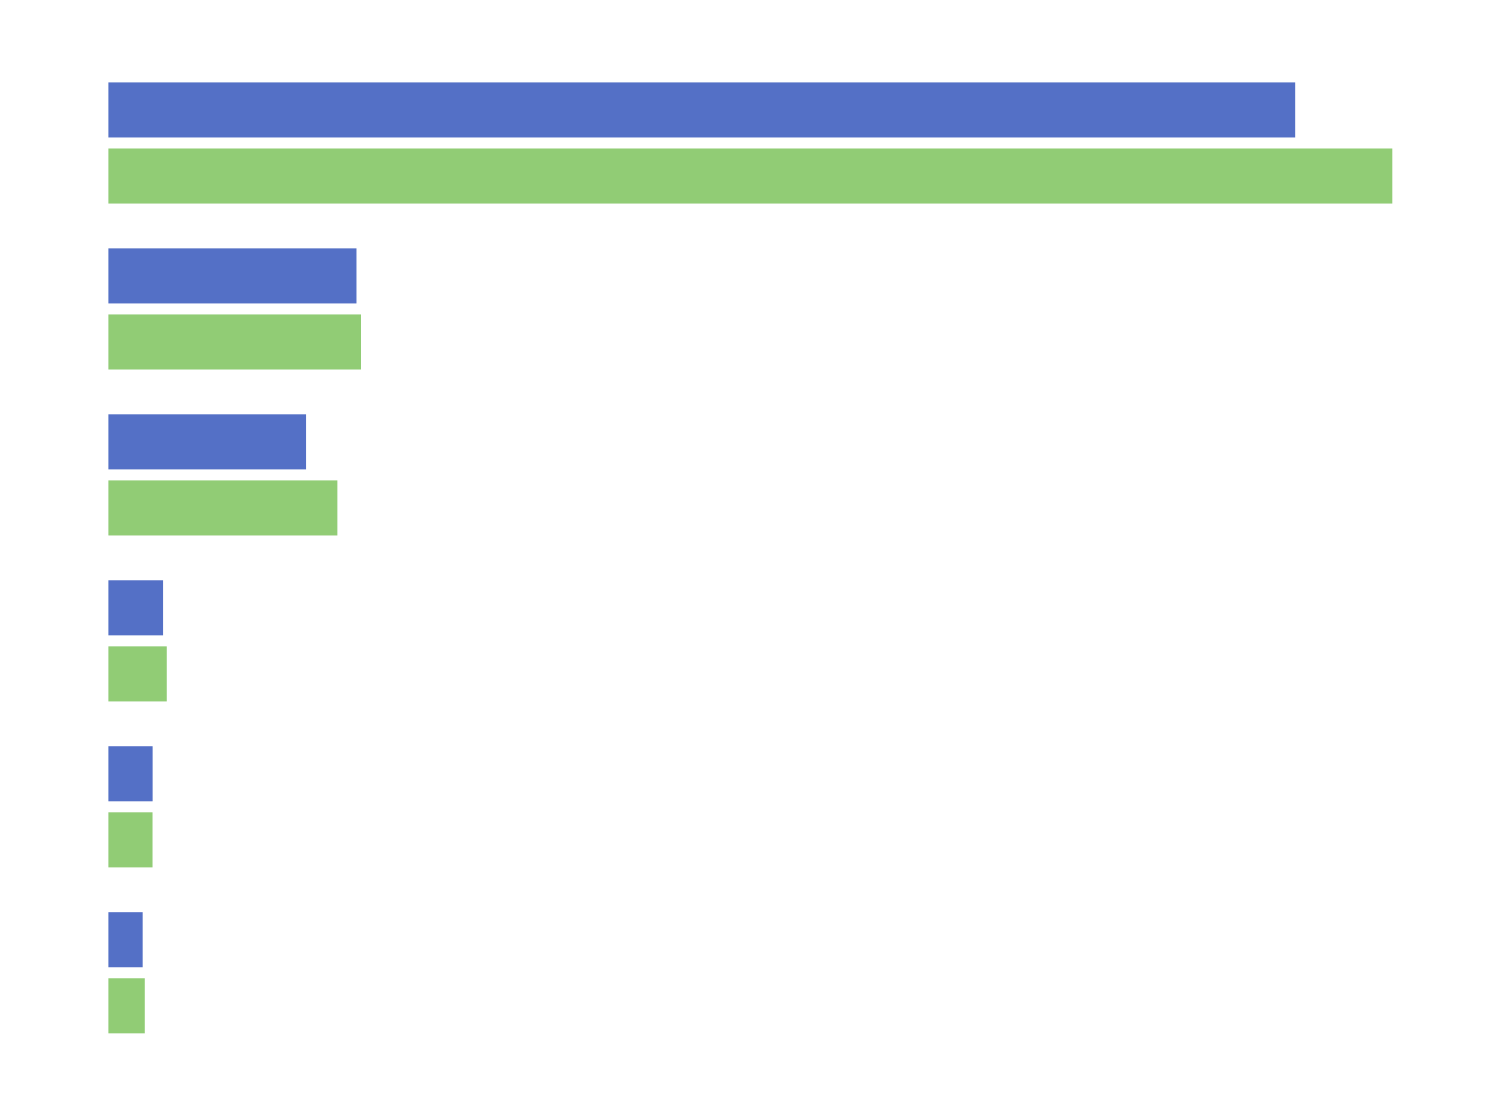
\includegraphics[width=\textwidth]{Train_set/6.pdf}
{6.svg (143.0)}
\end{minipage}
\hfill
\begin{minipage}{0.233\columnwidth}
\centering
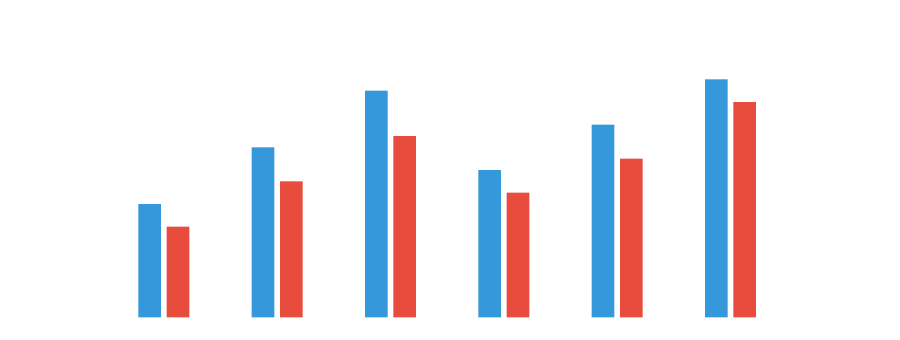
\includegraphics[width=\textwidth]{Train_set/7.pdf}
{7.svg (50.8)}
\end{minipage}
\hfill
\begin{minipage}{0.233\columnwidth}
\centering
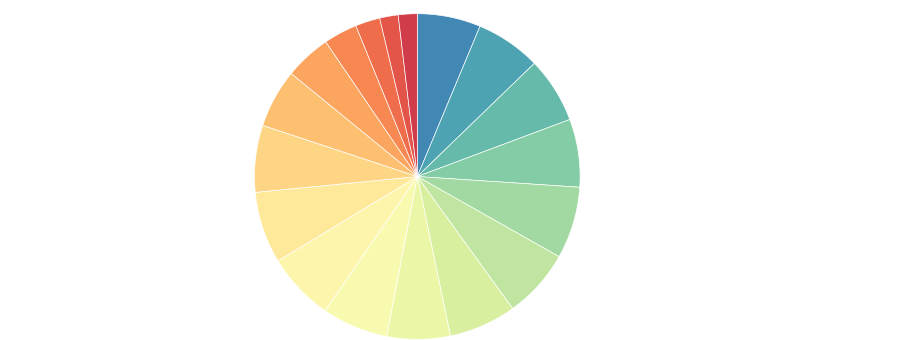
\includegraphics[width=\textwidth]{Train_set/8.pdf}
{8.svg (93.0)}
\end{minipage}
\end{figure}

\begin{figure}[!htbp]
\centering
\begin{minipage}{0.233\columnwidth}
\centering

\includegraphics[width=\textwidth]{Train_set/9.pdf}
{9.svg (163.2)}
\end{minipage}
\hfill
\begin{minipage}{0.233\columnwidth}
\centering

\includegraphics[width=\textwidth]{Train_set/10.pdf}
{10.svg (81.0)}
\end{minipage}
\hfill
\begin{minipage}{0.233\columnwidth}
\centering

\includegraphics[width=\textwidth]{Train_set/11.pdf}
{11.svg (386.5)}
\end{minipage}
\hfill
\begin{minipage}{0.233\columnwidth}
\centering
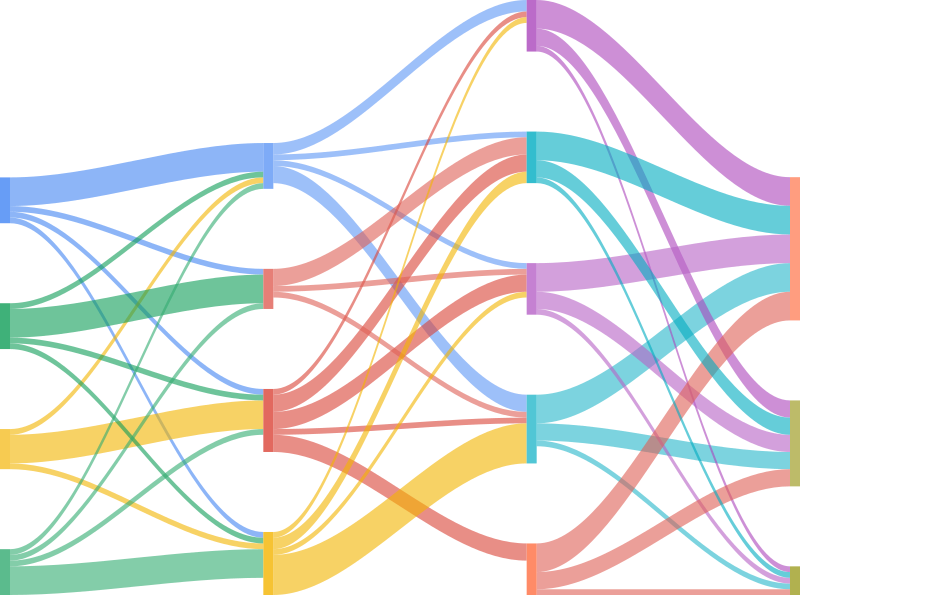
\includegraphics[width=\textwidth]{Train_set/12.pdf}
{12.svg (4684.0)}
\end{minipage}
\end{figure}

\begin{figure}[!htbp]
\centering
\begin{minipage}{0.233\columnwidth}
\centering
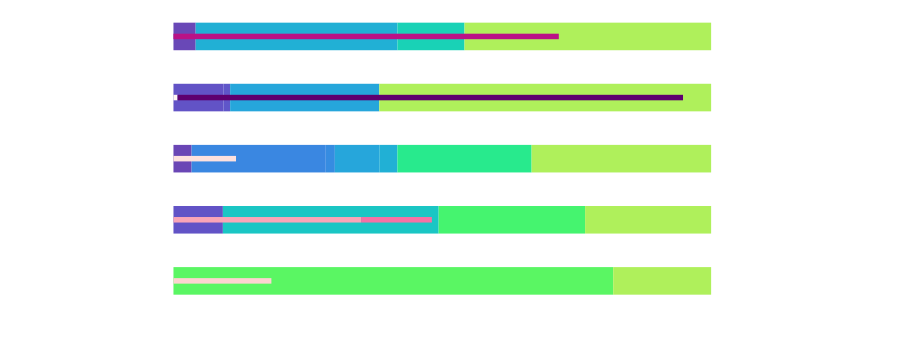
\includegraphics[width=\textwidth]{Train_set/13.pdf}
{13.svg (212.1)}
\end{minipage}
\hfill
\begin{minipage}{0.233\columnwidth}
\centering
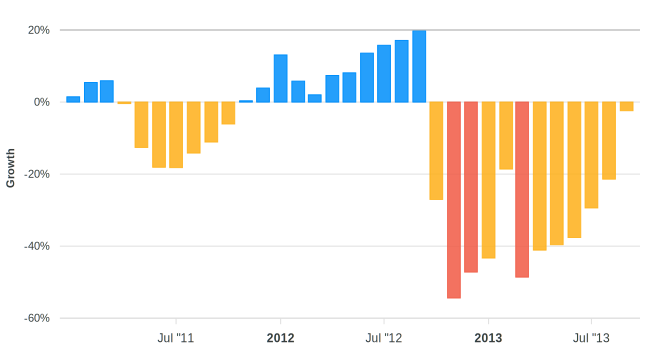
\includegraphics[width=\textwidth]{Train_set/14.pdf}
{14.svg (62.4)}
\end{minipage}
\hfill
\begin{minipage}{0.233\columnwidth}
\centering
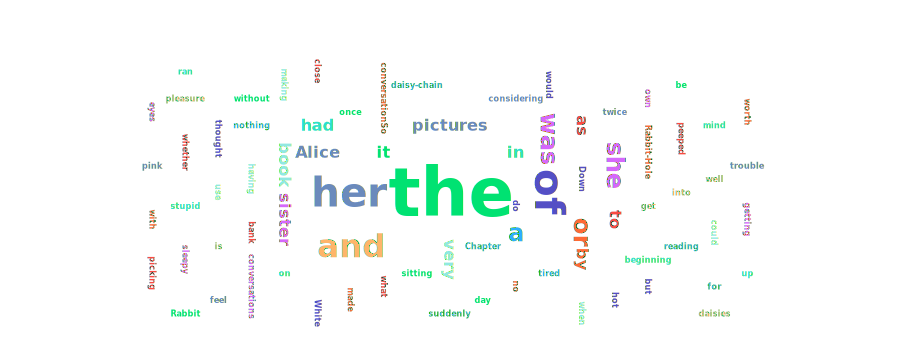
\includegraphics[width=\textwidth]{Train_set/15.pdf}
{15.svg (533.3)}
\end{minipage}
\hfill
\begin{minipage}{0.233\columnwidth}
\centering

\includegraphics[width=\textwidth]{Train_set/16.pdf}
{16.svg (187.3)}
\end{minipage}
\end{figure}

\begin{figure}[!htbp]
\centering
\begin{minipage}{0.233\columnwidth}
\centering
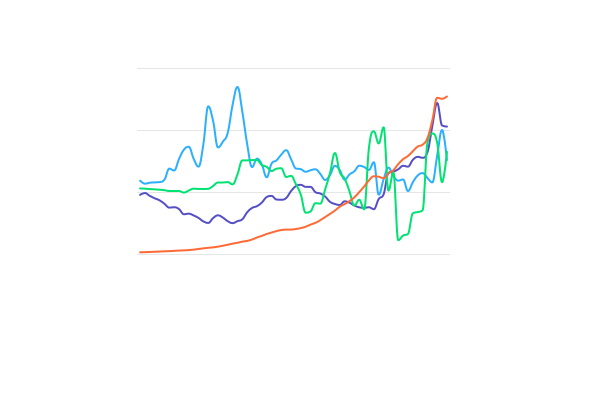
\includegraphics[width=\textwidth]{Train_set/17.pdf}
{17.svg (91.1)}
\end{minipage}
\hfill
\begin{minipage}{0.233\columnwidth}
\centering

\includegraphics[width=\textwidth]{Train_set/18.pdf}
{18.svg (394.0)}
\end{minipage}
\hfill
\begin{minipage}{0.233\columnwidth}
\centering
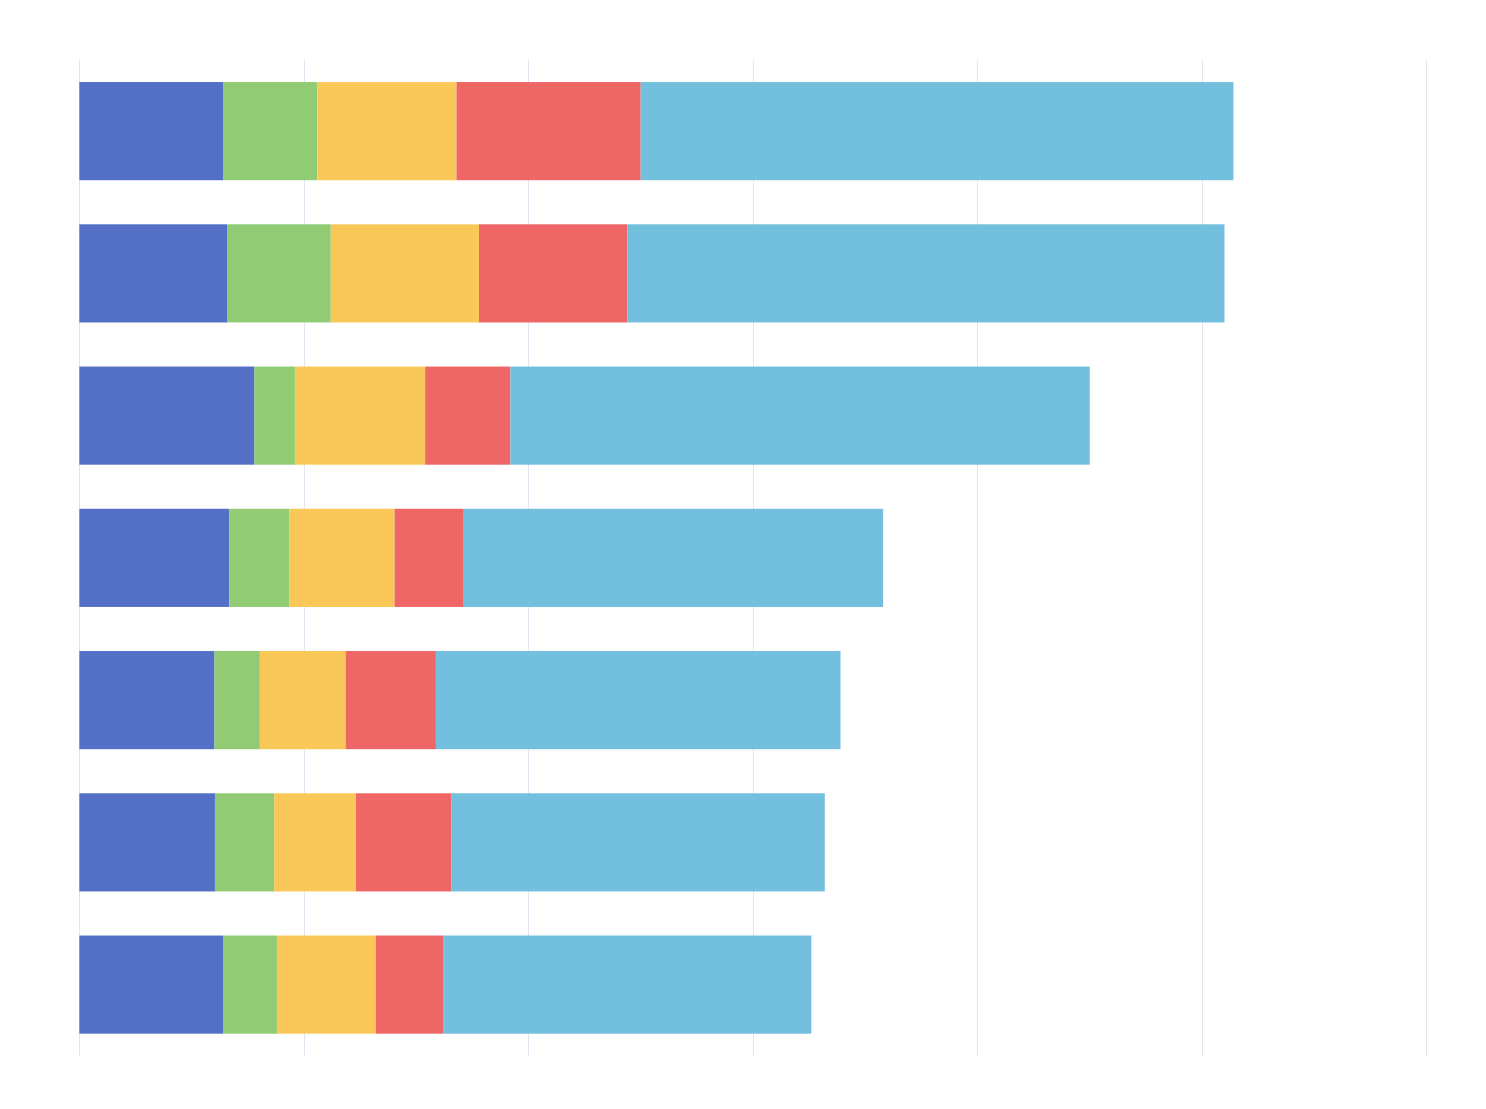
\includegraphics[width=\textwidth]{Train_set/19.pdf}
{19.svg (2093.8)}
\end{minipage}
\hfill
\begin{minipage}{0.233\columnwidth}
\centering

\includegraphics[width=\textwidth]{Train_set/20.pdf}
{20.svg (468.7)}
\end{minipage}
\end{figure}

\begin{figure}[!htbp]
\centering
\begin{minipage}{0.233\columnwidth}
\centering

\includegraphics[width=\textwidth]{Train_set/21.pdf}
{21.svg (94.9)}
\end{minipage}
\hfill
\begin{minipage}{0.233\columnwidth}
\centering
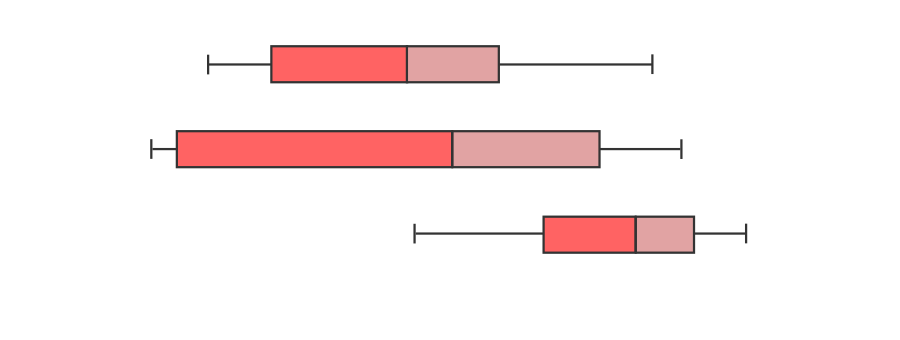
\includegraphics[width=\textwidth]{Train_set/22.pdf}
{22.svg (62.9)}
\end{minipage}
\hfill
\begin{minipage}{0.233\columnwidth}
\centering
\includegraphics[width=\textwidth]{Train_set/23.pdf}
{23.svg (216.7)}
\end{minipage}
\hfill
\begin{minipage}{0.233\columnwidth}
\centering
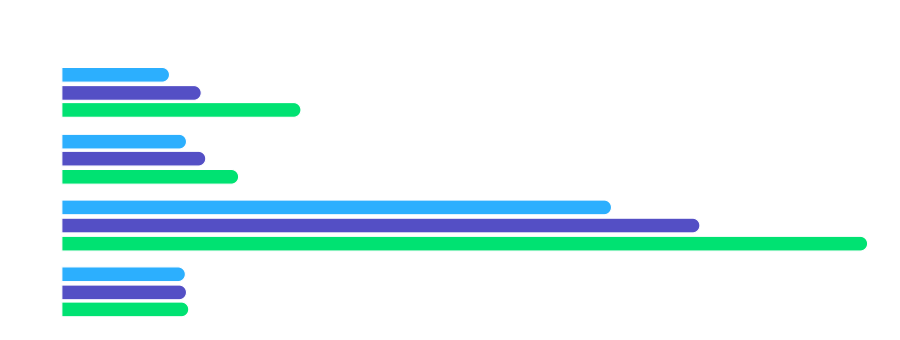
\includegraphics[width=\textwidth]{Train_set/24.pdf}
{24.svg (92.7)}
\end{minipage}
\end{figure}

\begin{figure}[!htbp]
\centering
\begin{minipage}{0.233\columnwidth}
\centering
\includegraphics[width=\textwidth]{Train_set/25.pdf}
{25.svg (98.9)}
\end{minipage}
\hfill
\begin{minipage}{0.233\columnwidth}
\centering
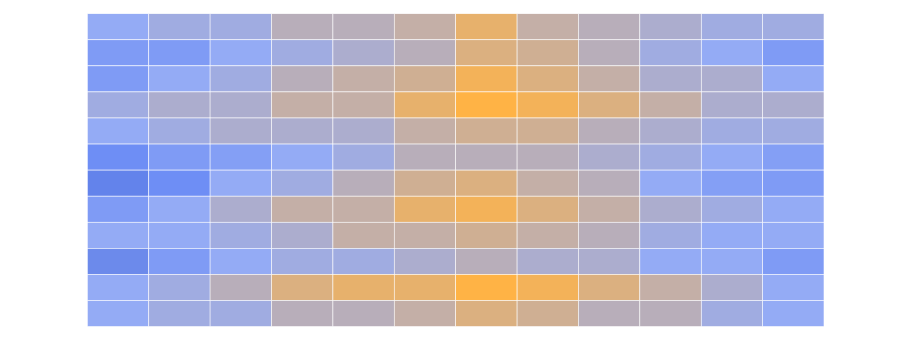
\includegraphics[width=\textwidth]{Train_set/26.pdf}
{26.svg (822.6)}
\end{minipage}
\hfill
\begin{minipage}{0.233\columnwidth}
\centering
\includegraphics[width=\textwidth]{Train_set/27.pdf}
{27.svg (384.8)}
\end{minipage}
\hfill
\begin{minipage}{0.233\columnwidth}
\centering

\includegraphics[width=\textwidth]{Train_set/28.pdf}
{28.svg (988.8)}
\end{minipage}
\end{figure}

\begin{figure}[!htbp]
\centering
\begin{minipage}{0.233\columnwidth}
\centering

\includegraphics[width=\textwidth]{Train_set/29.pdf}
{29.svg (73.3)}
\end{minipage}
\hfill
\begin{minipage}{0.233\columnwidth}
\centering
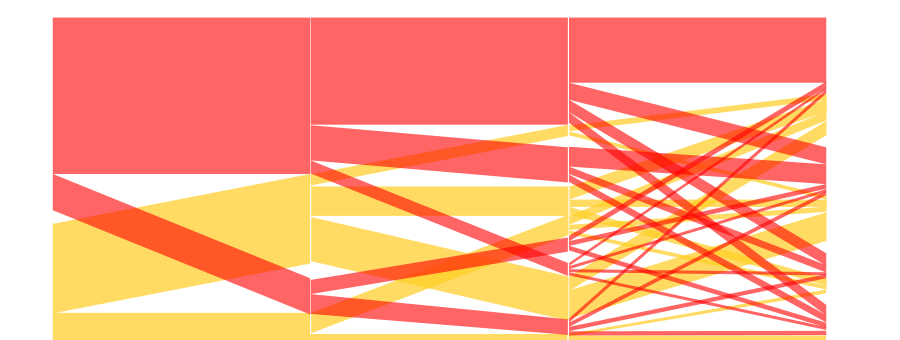
\includegraphics[width=\textwidth]{Train_set/30.pdf}
{30.svg (206.4)}
\end{minipage}
\hfill
\begin{minipage}{0.233\columnwidth}
\centering
\includegraphics[width=\textwidth]{Train_set/31.pdf}
{31.svg (77.0)}
\end{minipage}
\hfill
\begin{minipage}{0.233\columnwidth}
\centering

\includegraphics[width=\textwidth]{Train_set/32.pdf}
{32.svg (282.2)}
\end{minipage}
\end{figure}

\begin{figure}[!htbp]
\centering
\begin{minipage}{0.233\columnwidth}
\centering
\includegraphics[width=\textwidth]{Train_set/33.pdf}
{33.svg (1054.3)}
\end{minipage}
\hfill
\begin{minipage}{0.233\columnwidth}
\centering
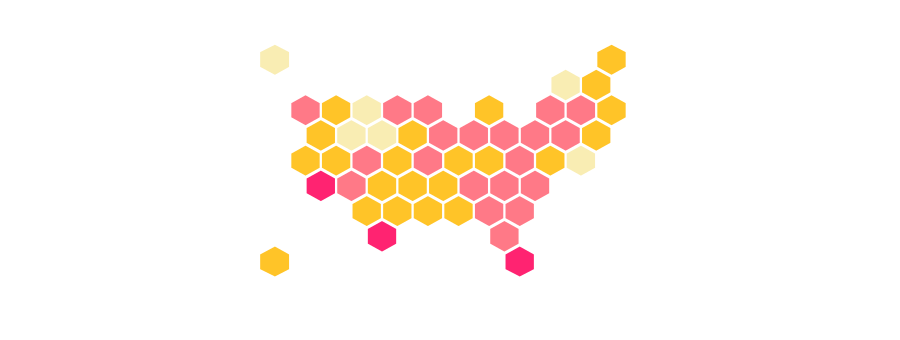
\includegraphics[width=\textwidth]{Train_set/34.pdf}
{34.svg (294.1)}
\end{minipage}
\hfill
\begin{minipage}{0.233\columnwidth}
\centering
\includegraphics[width=\textwidth]{Train_set/35.pdf}
{35.svg (587.8)}
\end{minipage}
\hfill
\begin{minipage}{0.233\columnwidth}
\centering
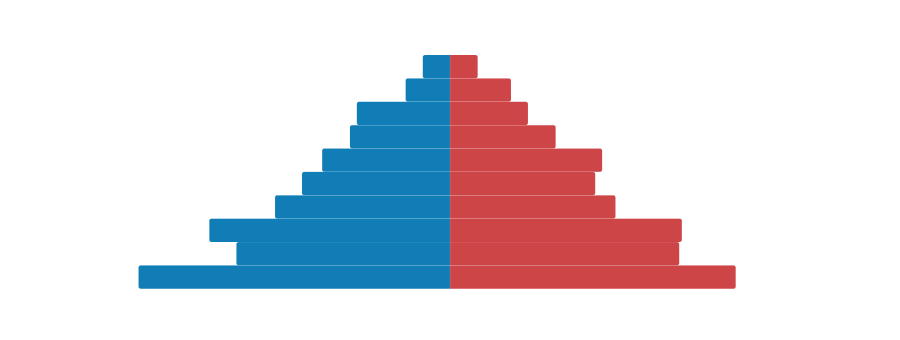
\includegraphics[width=\textwidth]{Train_set/36.pdf}
{36.svg (129.2)}
\end{minipage}
\end{figure}

\begin{figure}[!htbp]
\centering
\begin{minipage}{0.233\columnwidth}
\centering

\includegraphics[width=\textwidth]{Train_set/37.pdf}
{37.svg (366.0)}
\end{minipage}
\hfill
\begin{minipage}{0.233\columnwidth}
\centering

\includegraphics[width=\textwidth]{Train_set/38.pdf}
{38.svg (110.9)}
\end{minipage}
\hfill
\begin{minipage}{0.233\columnwidth}
\centering
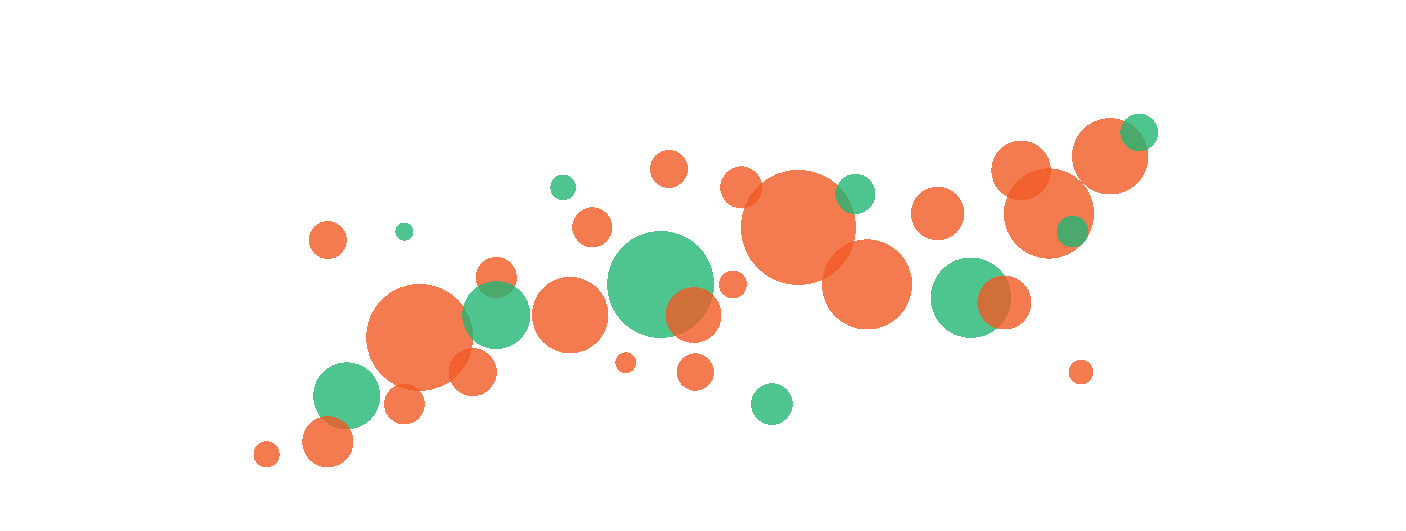
\includegraphics[width=\textwidth]{Train_set/39.pdf}
{39.svg (129.5)}
\end{minipage}
\hfill
\begin{minipage}{0.233\columnwidth}
\centering
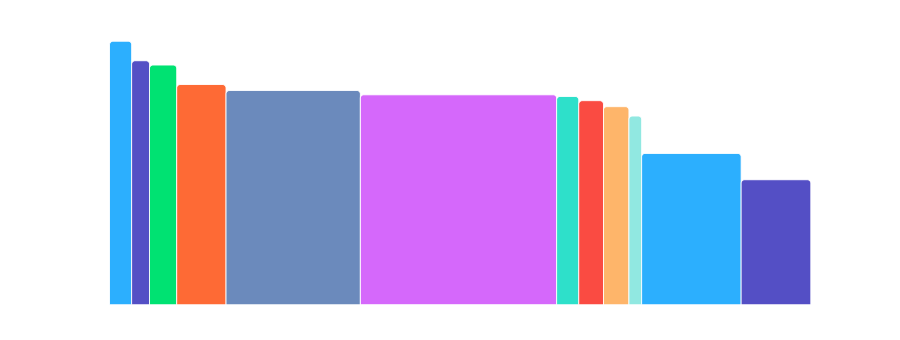
\includegraphics[width=\textwidth]{Train_set/40.pdf}
{40.svg (63.6)}
\end{minipage}
\end{figure}

\textbf{Test Set}

The following figures present all 20 test set visualizations ordered by filename for comprehensive reference and transparency.

\vspace{1em}

\begin{figure}[!htbp]
\centering
\begin{minipage}{0.233\columnwidth}
\centering
\includegraphics[width=\textwidth]{Test_set/1.pdf}
{1.svg (391.6)}
\end{minipage}
\hfill
\begin{minipage}{0.233\columnwidth}
\centering
\includegraphics[width=\textwidth]{Test_set/2.pdf}
{2.svg (136.6)}
\end{minipage}
\hfill
\begin{minipage}{0.233\columnwidth}
\centering

\includegraphics[width=\textwidth]{Test_set/3.pdf}
{3.svg (1752.6)}
\end{minipage}
\hfill
\begin{minipage}{0.233\columnwidth}
\centering
\includegraphics[width=\textwidth]{Test_set/4.pdf}
{4.svg (332.2)}
\end{minipage}
\end{figure}

\begin{figure}[!htbp]
\centering
\begin{minipage}{0.233\columnwidth}
\centering
\includegraphics[width=\textwidth]{Test_set/5.pdf}
{5.svg (102.3)}
\end{minipage}
\hfill
\begin{minipage}{0.233\columnwidth}
\centering
\includegraphics[width=\textwidth]{Test_set/6.pdf}
{6.svg (136.5)}
\end{minipage}
\hfill
\begin{minipage}{0.233\columnwidth}
\centering
\includegraphics[width=\textwidth]{Test_set/7.pdf}
{7.svg (3304.1)}
\end{minipage}
\hfill
\begin{minipage}{0.233\columnwidth}
\centering
\includegraphics[width=\textwidth]{Test_set/8.pdf}
{8.svg (1195.8)}
\end{minipage}
\end{figure}

\begin{figure}[!htbp]
\centering
\begin{minipage}{0.233\columnwidth}
\centering
\includegraphics[width=\textwidth]{Test_set/9.pdf}
{9.svg (84.1)}
\end{minipage}
\hfill
\begin{minipage}{0.233\columnwidth}
\centering
\includegraphics[width=\textwidth]{Test_set/10.pdf}
{10.svg (6627.5)}
\end{minipage}
\hfill
\begin{minipage}{0.233\columnwidth}
\centering
\includegraphics[width=\textwidth]{Test_set/11.pdf}
{11.svg (103.5)}
\end{minipage}
\hfill
\begin{minipage}{0.233\columnwidth}
\centering
\includegraphics[width=\textwidth]{Test_set/12.pdf}
{12.svg (127.9)}
\end{minipage}
\end{figure}

\begin{figure}[!htbp]
\centering
\begin{minipage}{0.233\columnwidth}
\centering
\includegraphics[width=\textwidth]{Test_set/13.pdf}
{13.svg (146.9)}
\end{minipage}
\hfill
\begin{minipage}{0.233\columnwidth}
\centering
\includegraphics[width=\textwidth]{Test_set/14.pdf}
{14.svg (175.5)}
\end{minipage}
\hfill
\begin{minipage}{0.233\columnwidth}
\centering
\includegraphics[width=\textwidth]{Test_set/15.pdf}
{15.svg (1214.1)}
\end{minipage}
\hfill
\begin{minipage}{0.233\columnwidth}
\centering
\includegraphics[width=\textwidth]{Test_set/16.pdf}
{16.svg (767.5)}
\end{minipage}
\end{figure}

\begin{figure}[!htbp]
\centering
\begin{minipage}{0.233\columnwidth}
\centering
\includegraphics[width=\textwidth]{Test_set/17.pdf}
{17.svg (953.0)}
\end{minipage}
\hfill
\begin{minipage}{0.233\columnwidth}
\centering
\includegraphics[width=\textwidth]{Test_set/18.pdf}
{18.svg (374.6)}
\end{minipage}
\hfill
\begin{minipage}{0.233\columnwidth}
\centering
\includegraphics[width=\textwidth]{Test_set/19.pdf}
{19.svg (213.1)}
\end{minipage}
\hfill
\begin{minipage}{0.233\columnwidth}
\centering
\includegraphics[width=\textwidth]{Test_set/20.pdf}
{20.svg (550.1)}
\end{minipage}
\end{figure}

\end{document} 

